\def\topic{Recursion}
\input{comp125lectureHeader}
\newpage

\begin{lstlisting}
public class Client {
	public static void main(String[] args) {
		int a = 4;
		int b = sum(a);
	}
	
	public static int sum(int n) {
		int result = n + sum(n-1);
		return result;
	}
}
\end{lstlisting}

\newpage

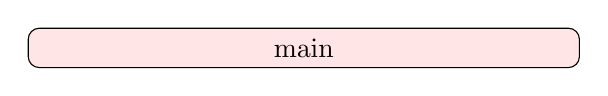
\begin{tikzpicture}
\scopeblock{functionName=main,variables={{"a=4","b=sum(4)"}},width=3.2}	
\draw[rounded corners,fill=red!10!white] (9,0) rectangle (16,0.5) node[pos=.5] {main};
\end{tikzpicture}
\vskip0.6cm

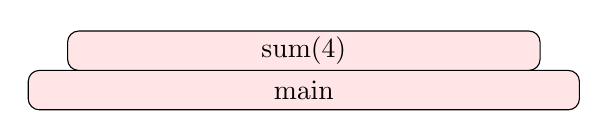
\begin{tikzpicture}
\scopeblock{functionName=main,variables={{"a=4","b=sum(4)"}},width=3.2}	
\scopeblock{x=5,functionName=sum(4),variables={{"n=4","result= 4 + sum(3)"}},width=3.2}
\arrow{startX=3,startY=2.3,endX=5.2,endY=2.3}
\draw[rounded corners,fill=red!10!white] (9,0) rectangle (16,0.5) node[pos=.5] {main};
\draw[rounded corners,fill=red!10!white] (9.5,0.5) rectangle (15.5,1) node[pos=.5] {sum(4)};
\end{tikzpicture}

\vskip0.6cm

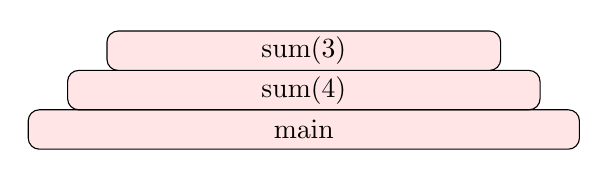
\begin{tikzpicture}
\scopeblock{functionName=sum(4),variables={{"n=4","result= 4 + sum(3)"}},width=3.2}
\scopeblock{x=5,functionName=sum(3),variables={{"n=3","result= 3 + sum(2)"}},width=3.2}
\arrow{startX=3,startY=2.3,endX=5.2,endY=2.3}
\draw[rounded corners,fill=red!10!white] (9,0) rectangle (16,0.5) node[pos=.5] {main};
\draw[rounded corners,fill=red!10!white] (9.5,0.5) rectangle (15.5,1) node[pos=.5] {sum(4)};
\draw[rounded corners,fill=red!10!white] (10,1) rectangle (15,1.5) node[pos=.5] {sum(3)};
\end{tikzpicture}

\vskip0.6cm

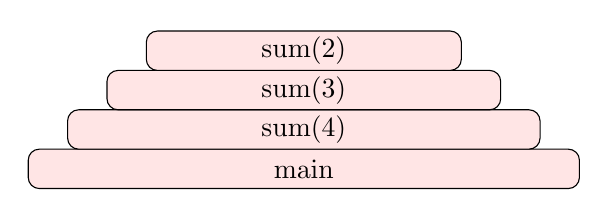
\begin{tikzpicture}
\scopeblock{functionName=sum(3),variables={{"n=3","result= 3 + sum(2)"}},width=3.2}
\scopeblock{x=5,functionName=sum(2),variables={{"n=2","result= 2 + sum(1)"}},width=3.2}
\arrow{startX=3,startY=2.3,endX=5.2,endY=2.3}
\draw[rounded corners,fill=red!10!white] (9,0) rectangle (16,0.5) node[pos=.5] {main};
\draw[rounded corners,fill=red!10!white] (9.5,0.5) rectangle (15.5,1) node[pos=.5] {sum(4)};
\draw[rounded corners,fill=red!10!white] (10,1) rectangle (15,1.5) node[pos=.5] {sum(3)};
\draw[rounded corners,fill=red!10!white] (10.5,1.5) rectangle (14.5,2) node[pos=.5] {sum(2)};
\end{tikzpicture}

\vskip0.6cm

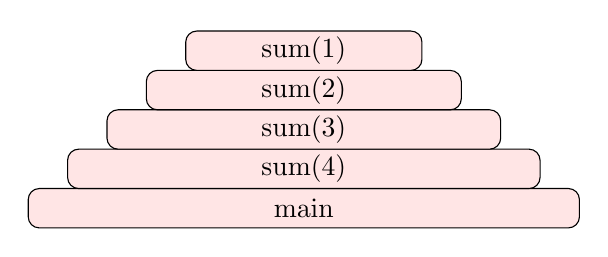
\begin{tikzpicture}
\scopeblock{functionName=sum(2),variables={{"n=2","result= 2 + sum(1)"}},width=3.2}
\scopeblock{x=5,functionName=sum(1),variables={{"n=1","result= 1 + sum(0)"}},width=3.2}
\arrow{startX=3,startY=2.3,endX=5.2,endY=2.3}
\draw[rounded corners,fill=red!10!white] (9,0) rectangle (16,0.5) node[pos=.5] {main};
\draw[rounded corners,fill=red!10!white] (9.5,0.5) rectangle (15.5,1) node[pos=.5] {sum(4)};
\draw[rounded corners,fill=red!10!white] (10,1) rectangle (15,1.5) node[pos=.5] {sum(3)};
\draw[rounded corners,fill=red!10!white] (10.5,1.5) rectangle (14.5,2) node[pos=.5] {sum(2)};
\draw[rounded corners,fill=red!10!white] (11,2) rectangle (14,2.5) node[pos=.5] {sum(1)};
\end{tikzpicture}

\vskip0.6cm

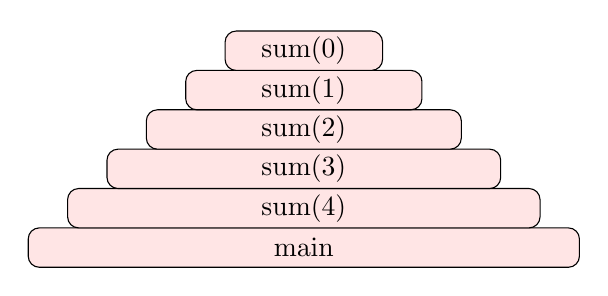
\begin{tikzpicture}
\scopeblock{functionName=sum(1),variables={{"n=1","result= 1 + sum(0)"}},width=3.2}
\scopeblock{x=5,functionName=sum(0),variables={{"n=0","result= 0"}},width=3.2}
\arrow{startX=3,startY=2.3,endX=5.2,endY=2.3}
\draw[rounded corners,fill=red!10!white] (9,0) rectangle (16,0.5) node[pos=.5] {main};
\draw[rounded corners,fill=red!10!white] (9.5,0.5) rectangle (15.5,1) node[pos=.5] {sum(4)};
\draw[rounded corners,fill=red!10!white] (10,1) rectangle (15,1.5) node[pos=.5] {sum(3)};
\draw[rounded corners,fill=red!10!white] (10.5,1.5) rectangle (14.5,2) node[pos=.5] {sum(2)};
\draw[rounded corners,fill=red!10!white] (11,2) rectangle (14,2.5) node[pos=.5] {sum(1)};
\draw[rounded corners,fill=red!10!white] (11.5,2.5) rectangle (13.5,3) node[pos=.5] {sum(0)};
\end{tikzpicture}

\vskip0.6cm

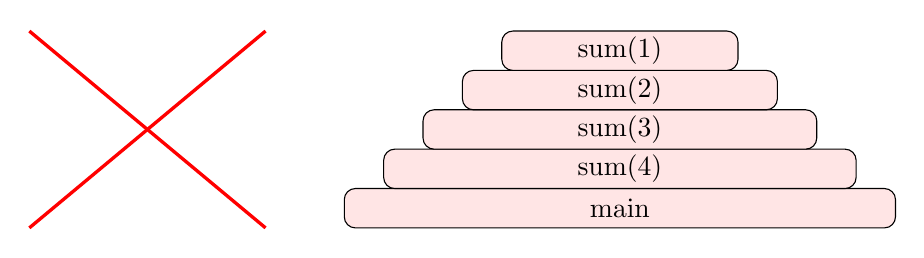
\begin{tikzpicture}
\scopeblock{functionName=sum(1),variables={{"n=1","result= 1 + sum(0)"}},width=3.2}
\scopeblock{x=5,functionName=sum(0),variables={{"n=0","result= 0"}},width=3.2}
\arrow{style=dashed,startX=5.2,startY=2.3,endX=2.8,endY=0.8,label=0}
\draw[red, very thick](5,2.5) -- (8,0);
\draw[red, very thick](5,0) -- (8,2.5);
\draw[rounded corners,fill=red!10!white] (9,0) rectangle (16,0.5) node[pos=.5] {main};
\draw[rounded corners,fill=red!10!white] (9.5,0.5) rectangle (15.5,1) node[pos=.5] {sum(4)};
\draw[rounded corners,fill=red!10!white] (10,1) rectangle (15,1.5) node[pos=.5] {sum(3)};
\draw[rounded corners,fill=red!10!white] (10.5,1.5) rectangle (14.5,2) node[pos=.5] {sum(2)};
\draw[rounded corners,fill=red!10!white] (11,2) rectangle (14,2.5) node[pos=.5] {sum(1)};
\end{tikzpicture}

\vskip0.6cm

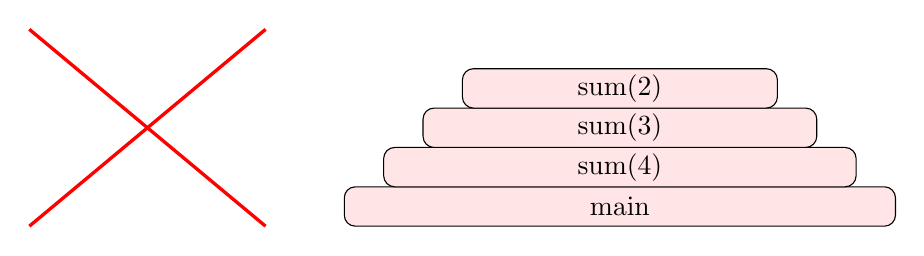
\begin{tikzpicture}
\scopeblock{functionName=sum(2),variables={{"n=2","result= 2 + sum(1)"}},width=3.2}
\scopeblock{x=5,functionName=sum(1),variables={{"n=1","result=1"}},width=3.2}
\arrow{style=dashed,startX=5.2,startY=2.3,endX=2.8,endY=0.8,label=1}
\draw[red, very thick](5,2.5) -- (8,0);
\draw[red, very thick](5,0) -- (8,2.5);
\draw[rounded corners,fill=red!10!white] (9,0) rectangle (16,0.5) node[pos=.5] {main};
\draw[rounded corners,fill=red!10!white] (9.5,0.5) rectangle (15.5,1) node[pos=.5] {sum(4)};
\draw[rounded corners,fill=red!10!white] (10,1) rectangle (15,1.5) node[pos=.5] {sum(3)};
\draw[rounded corners,fill=red!10!white] (10.5,1.5) rectangle (14.5,2) node[pos=.5] {sum(2)};
\end{tikzpicture}

\vskip0.6cm

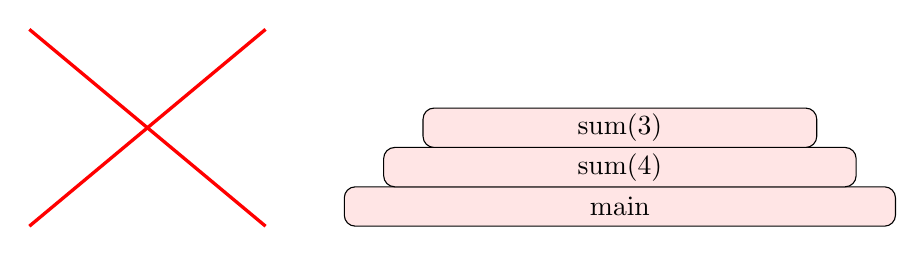
\begin{tikzpicture}
\scopeblock{functionName=sum(3),variables={{"n=3","result= 3 + sum(2)"}},width=3.2}
\scopeblock{x=5,functionName=sum(2),variables={{"n=2","result=3"}},width=3.2}
\arrow{style=dashed,startX=5.2,startY=2.3,endX=2.8,endY=0.8,label=3}
\draw[red, very thick](5,2.5) -- (8,0);
\draw[red, very thick](5,0) -- (8,2.5);
\draw[rounded corners,fill=red!10!white] (9,0) rectangle (16,0.5) node[pos=.5] {main};
\draw[rounded corners,fill=red!10!white] (9.5,0.5) rectangle (15.5,1) node[pos=.5] {sum(4)};
\draw[rounded corners,fill=red!10!white] (10,1) rectangle (15,1.5) node[pos=.5] {sum(3)};
\end{tikzpicture}

\vskip0.6cm

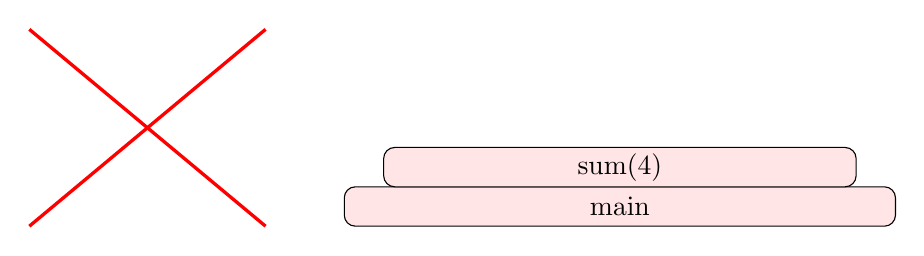
\begin{tikzpicture}
\scopeblock{functionName=sum(4),variables={{"n=4","result= 4 + sum(3)"}},width=3.2}
\scopeblock{x=5,functionName=sum(3),variables={{"n=3","result=6"}},width=3.2}
\arrow{style=dashed,startX=5.2,startY=2.3,endX=2.8,endY=0.8,label=6}
\draw[red, very thick](5,2.5) -- (8,0);
\draw[red, very thick](5,0) -- (8,2.5);
\draw[rounded corners,fill=red!10!white] (9,0) rectangle (16,0.5) node[pos=.5] {main};
\draw[rounded corners,fill=red!10!white] (9.5,0.5) rectangle (15.5,1) node[pos=.5] {sum(4)};
\end{tikzpicture}

\vskip0.6cm


\begin{tikzpicture}
\scopeblock{functionName=main,variables={{"a=4","b = sum(4)"}},width=3.2}	
\scopeblock{x=5,functionName=sum(4),variables={{"n=4","result=10"}},width=3.2}
\arrow{style=dashed,startX=5.2,startY=2.3,endX=2.8,endY=0.8,label=10}
\draw[red, very thick](5,2.5) -- (8,0);
\draw[red, very thick](5,0) -- (8,2.5);
\draw[rounded corners,fill=red!10!white] (9,0) rectangle (16,0.5) node[pos=.5] {main};
\end{tikzpicture}

\vskip0.6cm

\begin{tikzpicture}
\scopeblock{functionName=main,variables={{"a=4","b=10"}},width=3.2}	
\end{tikzpicture}

\input{comp125lectureFooter}